\documentclass{article}
\usepackage{iclr2026_conference,times}
% TODO: swap to the official ICLR 2027 style when released; anonymous submission (no \iclrfinalcopy)
\usepackage{graphicx,amsmath,amssymb,booktabs,multirow,xcolor,etoolbox}
\usepackage[pagebackref=false,breaklinks,colorlinks,citecolor=blue]{hyperref}
\newcommand{\mad}{madweight}
\renewcommand{\deg}{^{\circ}}

%%% ICLR DRAFT — evolving with incoming results. Integration log:
%%%  [x] RESfM baseline 3-seed band (s20-22) — Table 2 + band-language claims
%%%  [x] Extended tables: trans/rot/Nr panels (from 3DV supp Sec J)
%%%  [x] lr 2x2 grid + lr-robust vs lr-dependent OOD split (new Sec 5.2)
%%%  [x] ESFM* clean-track reference row (our star tracks)
%%%  [x] Registration two-notions + plain-remove coverage caveat
%%%  [x] 5-seed bands integrated (s20-24); OLSSON COLLAPSE = 4/5 SEEDS (conclusion change)
%%%  [x] uesfm@1e-3: loses everywhere at 1e-3 -> lr policy vindicated, asymmetry vs baseline (wttt fleet pending)
%%%  [x] 30k lr1e4: Ep16000 ckpt = near-parity MD (0.365) + keeps OOD gains; strongest supervised OOD variant
%%%  [x] faithful pair: authors' Accuracy selection weaker everywhere -> margins are lower bounds
%%%  [x] authors-faithful ESFM*: MD 0.462/0.049 (construction diff explained our-star 0.596); row updated
%%%  [ ] layer-norm deep multids RESfM baseline (job 914663-successor)
%%%  [ ] af-multids canonical-schedule replication; GLOMAP/Theia baselines
%%%  [ ] natbib citations; appendix = per-seed tables + reproducibility study

\title{SS-RESfM: Self-Supervised Outlier Handling\\
Across Contamination Regimes in Deep Structure-from-Motion}
\author{Anonymous authors\\Paper under double-blind review}

\begin{document}
\maketitle

\begin{abstract}
State-of-the-art deep equivariant Structure-from-Motion (RESfM) rejects outlier
correspondences with a \emph{supervised} classifier trained on COLMAP-derived labels. We
present \textbf{SS-RESfM}, an \emph{entirely self-supervised} alternative: the outlier
head is trained on confident pseudo-labels formed from percentiles of the model's own
reprojection error, and no ground-truth or COLMAP labels are used anywhere in training or
test. Under a strictly controlled protocol (identical tracks, robust bundle adjustment,
and training schedule, varying only the outlier mechanism) we compare label-free
statistical removal (\mad{}) and soft reweighting against a from-scratch RESfM baseline
across six datasets spanning $0.5\%$--$61\%$ measured outliers. The optimal mechanism
\emph{flips with contamination}. Removal wins the high-contamination regime: at $61\%$
plain removal beats the supervised baseline on every seed pair over five seeds each
($12.4\pm2.1$ vs.\ $19.2\pm3.4$) and both beat COLMAP, while at $43\%$ it beats every
supervised seed's median ($1.4$--$1.9$ vs.\ $2.4$--$4.3$). Reweighting wins the low-contamination regime, beating
the supervised baseline $2.6$--$3.8\times$ on clean out-of-distribution data. Supervision
retains the in-distribution regime and the cleanest OOD mean (self-supervised arms within
$\sim\!13$--$23\%$ in distribution). We trace this to a structural circularity: outlier labels
require a trusted reconstruction of the very scenes whose contamination makes
reconstruction hard (for \emph{any} gold-standard labeler, not just COLMAP), and we
measure the resulting \emph{label ceiling}: regenerating supervision from scratch, label
recall collapses from $0.82$ to $\sim\!0.3$ above $\sim\!15\%$ contamination, precisely
where robustness is needed. Label-free adaptivity is thus a missing ingredient for robust
deep SfM.
\end{abstract}

\section{Introduction}
Structure-from-Motion (SfM) recovers camera poses and 3D structure from unordered image
collections. Its correspondences are heavily contaminated by outliers (wrong matches
that survive pairwise geometric verification), particularly in Internet photo collections
where repeated and symmetric structure produces spurious epipolar geometries. Classical
pipelines reject outliers with RANSAC and robust bundle adjustment (BA); recent deep
equivariant methods (ESFM~\cite{esfm}, RESfM~\cite{resfm}) instead learn a
\emph{sets-of-sets} permutation-equivariant network that regresses cameras from point
tracks and, in RESfM, adds a supervised per-point \emph{inlier/outlier classification
module}. RESfM's labels are derived from a COLMAP~\cite{colmap} reconstruction in two
stages: first by track membership, then refined by a $4$-pixel reprojection test against
COLMAP-pose triangulation~\cite{resfm}.

We take a different route. Rather than supervise the head with COLMAP labels, \textbf{SS-RESfM}
trains it \emph{self-supervised}: an adaptive confidence-weighted loss forms confident
pseudo-labels from percentiles of the model's own reprojection error, so no ground-truth or
COLMAP outlier labels are used anywhere in training or test. On top of this self-supervised
head we study a question RESfM's single supervised mechanism leaves open: \emph{is one
outlier-handling mechanism optimal across the range of contamination levels SfM encounters?}
We find that it is not. Holding everything else fixed and varying \emph{only} the
outlier-handling mechanism, the best mechanism \textbf{flips with contamination}:
hard removal at high contamination, soft reweighting at low, with the supervised
classifier retaining the typical in-distribution scene and the cleanest OOD mean
(Fig.~\ref{fig:complement}).
We further show the removal family wins the high-contamination regime outright: plain
removal beats the supervised baseline on every seed at both $43\%$ and $\sim\!60\%$,
while \mad{}, which discards points by the median-absolute-deviation (MAD) of their
reprojection error and soft-weights the survivors with no learned threshold, matches the
baseline there and beats COLMAP. We attribute this to
(i)~domain shift, since the classifier is trained only on in-distribution MegaDepth, and
(ii)~supervised labeling's dependence on a COLMAP reconstruction and ground-truth poses,
readily obtained for curated data but not for the contaminated collections where
robustness is most needed; a label-free, per-scene mechanism is attractive precisely
in that regime.

The appeal of self-supervision here is structural, not incidental. Outlier labels must be
derived from a trusted reconstruction of the very scenes whose contamination makes
reconstruction hard, so supervision bootstraps from precisely the capability it is meant
to provide. This circularity is not specific to COLMAP: \emph{any} gold-standard labeler
must first solve the scene in order to label its outliers, and it is exactly the
challenging, contaminated collections that defeat this bootstrapping. A self-supervised
head, by contrast, consumes only the point tracks themselves; the training data for robust
SfM then becomes as unlimited as unlabeled imagery, and new domains require no labeling
infrastructure at all.

\noindent\textbf{Contributions.}
(1)~\textbf{SS-RESfM, an entirely self-supervised outlier-handling approach} for deep SfM: an
adaptive confident-pseudo-label head (trained on percentiles of the model's own reprojection
error), label-free statistical removal, and robust BA, using \emph{no} ground-truth or
COLMAP outlier labels, in contrast to RESfM's COLMAP-supervised head. It beats the
supervised baseline on clean out-of-distribution data and at high contamination.
(2)~A controlled study of label-free removal vs.\ soft reweighting
($\pm$test-time fine-tuning) under an identical tracks\,+\,BA\,+\,schedule pipeline,
isolating the mechanism alone.
(3)~The complementarity finding: the optimal mechanism flips with contamination; no single
mechanism dominates.
(4)~\mad{}, which removes outliers by robust reprojection statistics (MAD), needing not
even the head, and reweights survivors; it matches the from-scratch supervised baseline at
extreme contamination ($\sim\!60\%$) with no learned threshold, while plain removal on
the same self-supervised head beats the baseline outright, and both beat COLMAP, which
registers only two-thirds of the cameras.

\section{Related Work}
\textbf{Deep equivariant SfM.} Learning-based SfM regresses cameras from point tracks with
permutation-equivariant networks. ESFM~\cite{esfm} casts uncalibrated SfM as deep projective
factorization over a measurement tensor, trained with an unsupervised reprojection loss;
GASFM~\cite{gasfm} uses a graph-attention variant. Both assume outliers were already removed
by two-view geometric verification. RESfM~\cite{resfm} targets contaminated internet
collections with a \emph{sets-of-sets} architecture plus a supervised per-point
inlier/outlier classification module and a robust BA, reporting accuracy close to its own
clean-track upper bound (``ESFM$^\ast$'') and on par with classical Theia/GLOMAP
(often with better translation recovery, while registering fewer images).
End-to-end pointmap and pose-regression pipelines (VGGSfM, MASt3R, DUSt3R) target far
smaller image sets. We propose no new architecture; we reuse the RESfM/ESFM backbone and
study the outlier-handling stage in isolation.

\noindent\textbf{Outlier rejection.} Correspondence outliers that \emph{survive}
RANSAC/two-view filtering are the central difficulty in internet-scale SfM. Classical
pipelines suppress them with M-estimators and robust BA; RESfM casts rejection as
supervised classification. We contrast supervised classification against \emph{label-free}
statistical removal via the median absolute deviation (MAD)~\cite{mad} and soft
reweighting, and show their relative merit is contamination-dependent.

\noindent\textbf{Robust bundle adjustment.} Following~\cite{resfm}, we apply a robust BA
that removes high-reprojection and low-visibility points, keeps the largest connected
component, re-triangulates, and re-optimizes. This stage is identical across all our arms.

\noindent\textbf{Test-time adaptation.} Per-scene fine-tuning at inference is used by ESFM/
RESfM to reach sub-pixel accuracy. We treat it as an orthogonal option ($\pm$TTT) applied
uniformly across mechanisms.

\section{Method}
\subsection{Background}
The input is a (sparse) point-track tensor $M$ of $m$ tracks across $n$ cameras, built by
concatenating pairwise RANSAC-verified SIFT matches. The sets-of-sets permutation-equivariant
network~\cite{resfm,esfm} maps $M$ to per-camera poses and a \emph{per-point} outlier score
$s\in[0,1]$ (points in the same track may receive different scores). Crucially, unlike RESfM,
whose classification head is trained with a BCE loss against \emph{COLMAP-derived}
inlier/outlier labels, SS-RESfM trains this head \emph{self-supervised}, with an adaptive
confidence-weighted loss: per forward pass it forms confident pseudo-labels from percentiles
of the model's own reprojection error (lowest $p$\% inliers, highest $p$\% outliers) and
applies BCE only to those. No ground-truth or COLMAP outlier labels are used at any point.
A reprojection error $e$ is available for every observation once an initial reconstruction
exists. All mechanisms below consume $s$ (and, for \mad{}, $e$),
produce a per-observation weight $w$ (or a hard keep/drop decision), and feed the result to
the identical robust-BA stage (Fig.~\ref{fig:method}).

\subsection{Outlier-handling mechanisms}
We compare four mechanisms, illustrated as weight-vs-signal transfer functions in
Fig.~\ref{fig:method}:
\begin{itemize}\itemsep2pt
\item\textbf{remove} (the RESfM analogue): drop a point if $s>\tau$; keep with $w{=}1$
otherwise. We use RESfM's default $\tau{=}0.6$ and its $\tau{=}0.8$ for the low-outlier,
single-camera Strecha/BlendedMVS sets~\cite{resfm}.
\item\textbf{weight}: soft, $w=1-s$, no removal.
\item\textbf{hybrid}: three-band: keep ($s$ below a low percentile), soft-weight (middle),
drop ($s$ above a high percentile).
\item\textbf{\mad{}} (ours): removal is driven by robust \emph{reprojection} statistics, not
the head. An observation is removed if its reprojection error exceeds
$\mathrm{med}(e)+\alpha\cdot\mathrm{MAD}(e)$ ($\alpha{=}2$); surviving observations are
soft-weighted by $w=1-s$. \mad{} is the only mechanism that consumes the reprojection
branch $e$ and requires \emph{no} learned threshold for removal.
\end{itemize}
Each mechanism is evaluated with and without test-time fine-tuning ($\pm$TTT), in which the
head continues to adapt on the test scene.

\subsection{Test-time fine-tuning and robust BA}
We load a multi-scene checkpoint, run a per-scene forward pass to obtain $s$ and $e$, apply
the mechanism, fine-tune per scene ($\sim\!1000$ iterations) under the reprojection
objective, and apply robust BA. This protocol, the seed, and the schedule are held fixed
across all arms; only the mechanism block changes.

\section{Experiments}
\subsection{Datasets and contamination}
We evaluate on six datasets spanning a wide contamination range. Alongside the RESfM
paper's quoted outlier fractions we report the contamination \emph{measured on our own
tracks} (robust ground-truth-pose triangulation with the standard $4$px cutoff, applied
uniformly to every dataset); see Table~\ref{tab:datasets}.
\begin{table}[t]\centering\footnotesize
\caption{\textbf{Datasets}: outlier rates (RESfM-reported vs.\ measured on our tracks) and regime.}
\label{tab:datasets}
\setlength{\tabcolsep}{1.2pt}%
\begin{tabular}{lccc}
\toprule
Dataset & RESfM\% & ours\% & Regime\\
\midrule
Strecha~\cite{strecha} & 2.7 & 1.7 & clean, LIDAR GT\\
BlendedMVS~\cite{blendedmvs} & 3.6 & 3.1 & low-outlier\\
MegaDepth~\cite{megadepth} & 25.6 & 25.4 & contam., \emph{in-dist.}\\
1DSfM~\cite{onedsfm} & 31.9 & 43.3 & contam., OOD\\
1DSfM-hard & -- & $\sim$60 & extreme, OOD\\
Olsson~\cite{olsson} & -- & 0.5 & outlier-free\\
\bottomrule
\end{tabular}
\end{table}
On MegaDepth (where tracks are identical to RESfM's) the two measurements agree
($25.4$ vs $25.6$), validating our measurement; our 1DSfM rebuild is markedly harder than
the tracks behind RESfM's quoted $31.9\%$, which should be kept in mind when reading the
1DSfM columns. \emph{1DSfM-hard} comprises the five 1DSfM scenes unused by the standard
ten-scene split (Gendarmenmarkt, Piccadilly, Roman Forum, Trafalgar, Union Square), built
with the same pipeline and subsampled to $300$ cameras per scene following RESfM's
convention. Networks are trained on 27 MegaDepth scenes; MegaDepth test is therefore
in-distribution, while 1DSfM/1DSfM-hard/Strecha/BlendedMVS/Olsson are cross-dataset
(out-of-distribution).

\subsection{Protocol, baselines, and track provenance}\label{sec:protocol}
Following RESfM's public training code and default configuration, all networks train for
$20{,}000$ epochs with seed $20$ (the seed reported by RESfM~\cite{resfm}) as the primary
seed; the self-supervised arms are additionally replicated with seeds $21$/$22$, and cells
marked $^{\ddagger}$ report mean$\pm$std over the three seeds, \emph{including the
supervised baseline}, whose own seed band is reported throughout (its MegaDepth mean is
notably seed-volatile, $0.32\pm0.12$, while its median is stable, $0.06\pm0.01$). Batch size,
image subsampling, the eleven-milestone learning-rate decay schedule
($10\mathrm{k},11\mathrm{k},\dots,20\mathrm{k}$, $\gamma{=}0.9$), and validation-based
early stopping follow that released configuration and are held identical across all arms.
Two deliberate settings are disclosed. First, the \emph{base} learning rate is per-method:
$10^{-3}$ for the supervised arms (RESfM's released value) and $10^{-4}$ for the
self-supervised arms, whose adaptive pseudo-label loss converges early (best checkpoint by
epoch ${\sim}7.5$k, \emph{before} the first decay milestone; the supervised arms peak at
epoch ${\sim}16.5$k); both are well within the budget, so neither method is
truncation-limited. Second, two secondary values (the infinity-point margin and the
validation metric used for checkpoint selection) are held \emph{identical across all arms}
rather than at RESfM's released values, preserving the controlled comparison. The
selection deviation demonstrably \emph{favors} the baseline: under the authors' own
Accuracy-based checkpoint selection the supervised baseline is weaker on every dataset
(RESfM-faithful row in Table~\ref{tab:main}; MegaDepth $0.50$ vs.\ $0.34$), so all
reported supervised-baseline margins are lower bounds, and the baseline's clean-benchmark
failures persist under its own selection rule (Olsson $8.8$, BlendedMVS rotation
$53\deg$). We report two
architectures: shallow ($1{\times}3$) and deep ($2{\times}3$).

\noindent\textbf{Fair-comparison anchor.} Our controlled baseline is
\emph{RESfM-from-scratch}: trained by us with the \emph{identical} setup as our arms (same
27 scenes, sampling, epochs, seed), so only the outlier mechanism differs. We additionally
report \emph{RESfM-released} (authors' weights) and \emph{RESfM (paper)}.\footnote{The
ESFM row likewise follows the unified $20$k-epoch protocol. ESFM's own released
multi-scene (calibrated) recipe trains for $30$k epochs plus a $500$-epoch per-scene
fine-tune; we deliberately hold the schedule fixed across all rows so that the outlier
mechanism remains the only controlled variable.}

\noindent\textbf{Track provenance.} MegaDepth tracks, preprocessing, and the 36 test scenes
are \emph{identical} to RESfM, so MegaDepth is directly comparable to published numbers. The
OOD tracks (1DSfM/1DSfM-hard/Strecha/BlendedMVS/Olsson) are \emph{built by us} from the
publicly released images and ground truth (feature extraction, matching, and track
formation with our pipeline; RESfM did not release OOD tracks); OOD comparisons are therefore \emph{controlled within our pipeline} and are
\textbf{not} directly comparable to RESfM's published OOD numbers. On MegaDepth, RESfM's
own released weights yield $0.209$ in our harness (vs.\ their reported $0.169$),
confirming our evaluation is faithful and that $\sim\!0.209$ is the reproducible level;
this is unchanged ($0.217$) under the authors' exact pinned software stack (MKL BLAS,
same pycolmap/pyceres), isolating the residual gap to solver/hardware-level
nondeterminism in robust BA (analysis in the appendix). All reported results come from this
single pipeline and software stack; a stack-replication study (appendix) shows the
no-TTT arms are insensitive to it, while test-time fine-tuned \emph{means} inherit
solver-level nondeterminism and should be read with that variance in mind.

\noindent\textbf{Schedule robustness.} All reported results use RESfM's released
eleven-milestone schedule. An earlier accidental five-milestone variant of ours was
retired; a three-seed replication of \emph{both} schedules shows the schedule effect lies
within seed noise (MegaDepth $0.46\pm0.08$ vs.\ $0.40\pm0.09$; 1DSfM $9.6\pm3.2$ vs.\
$12.2\pm2.4$, per-seed rankings inverting on both), with mechanism orderings stable
throughout.

\noindent\textbf{A method-isolated comparison, not a SOTA claim.} Because
RESfM-from-scratch shares every pipeline component with our arms and differs only in the
outlier mechanism, it isolates the effect of removing supervision, the same controlled
protocol RESfM itself uses when it re-trains ESFM/GASFM in its own pipeline. We do
\emph{not} claim state of the art: RESfM's \emph{released} checkpoint ($0.209$ on
MegaDepth) is stronger than either from-scratch arm. This reproduction gap stems from the
released weights themselves, not our pipeline (the authors' \emph{own} training code on
our tracks reproduces $0.34$--$0.39$, not $0.209$), so it handicaps the
supervised and self-supervised arms \emph{equally}. We report RESfM-released and
RESfM~(paper) as reference rows throughout.

\noindent\textbf{Metrics.} Following RESfM's convention we draw conclusions from
\emph{mean} errors (translation emphasized, rotation reported alongside), post-BA
(rotation in degrees; translation is the aligned camera-position error in scene
coordinates), and provide medians as supporting statistics (RESfM likewise reports
medians in its appendix). The one declared exception is 1DSfM, whose mean is dominated by
two symmetric-structure failure scenes (Ellis Island, Tower of London) that fail for
\emph{all} methods; there we treat the median as the representative figure. Rotation and
registered-camera counts ($N_r$) for all arms are tabulated in the supplementary
(appendix); rotation broadly agrees with translation (the supervised BlendedMVS failure
is even larger in rotation), and under high contamination the label-free arms register
\emph{more} cameras than the supervised baseline ($38$--$43\%$ vs.\ $37\%$ of
ground-truth cameras on 1DSfM-hard). Two registration notions must be distinguished:
every learned arm outputs a pose for every camera (pose coverage; COLMAP genuinely fails
on $36\%$ of 1DSfM-hard), while $N_r$ counts the cameras surviving robust BA and a
$5$-pixel quality mask, the set over which errors are computed. Under this stricter
notion the plain-removal arms attain their low errors over a reduced set ($59\%$/$28\%$
vs.\ the baseline's $77\%$/$37\%$ on 1DSfM/1DSfM-hard), consistent with aggressive
pruning disconnecting weakly-supported cameras; \mad{} is registration-matched to the
baseline ($74\%$/$38\%$), so its comparisons are not coverage artifacts.

\begin{figure*}[t]
\centering
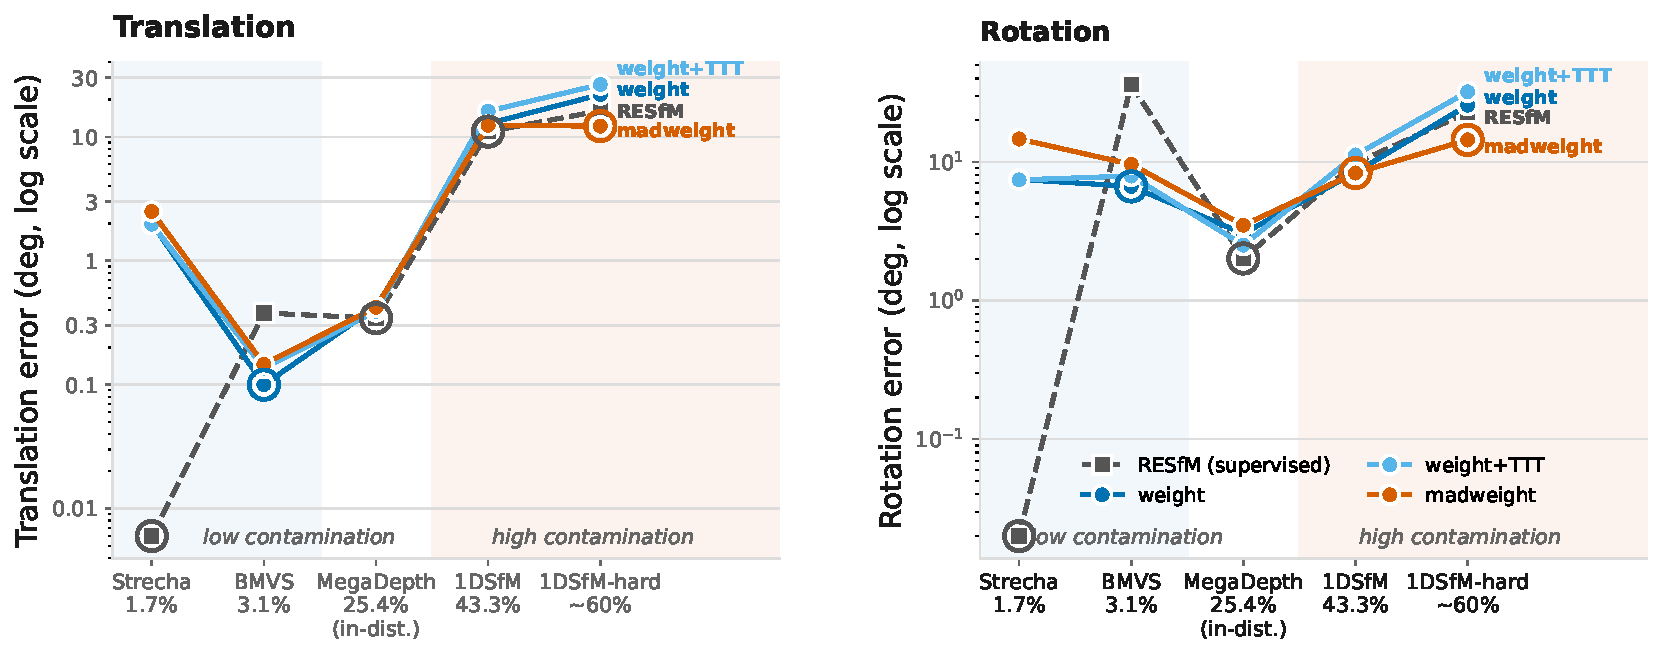
\includegraphics[width=0.92\textwidth]{PATHA_fig1_complementarity.pdf}
\caption{\textbf{The optimal outlier mechanism flips with contamination.} Translation
(left) and rotation (right) means (log scale) of the self-supervised arms vs.\ supervised
RESfM, five of the six datasets ordered by measured contamination
(Table~\ref{tab:main} data). Circled = best per dataset. The rotation panel mirrors the
translation ordering, with a self-supervised arm best on 1DSfM and the supervised
BlendedMVS failure even more pronounced ($36\deg$).}
\label{fig:complement}
\end{figure*}

\begin{figure*}[t]
\centering
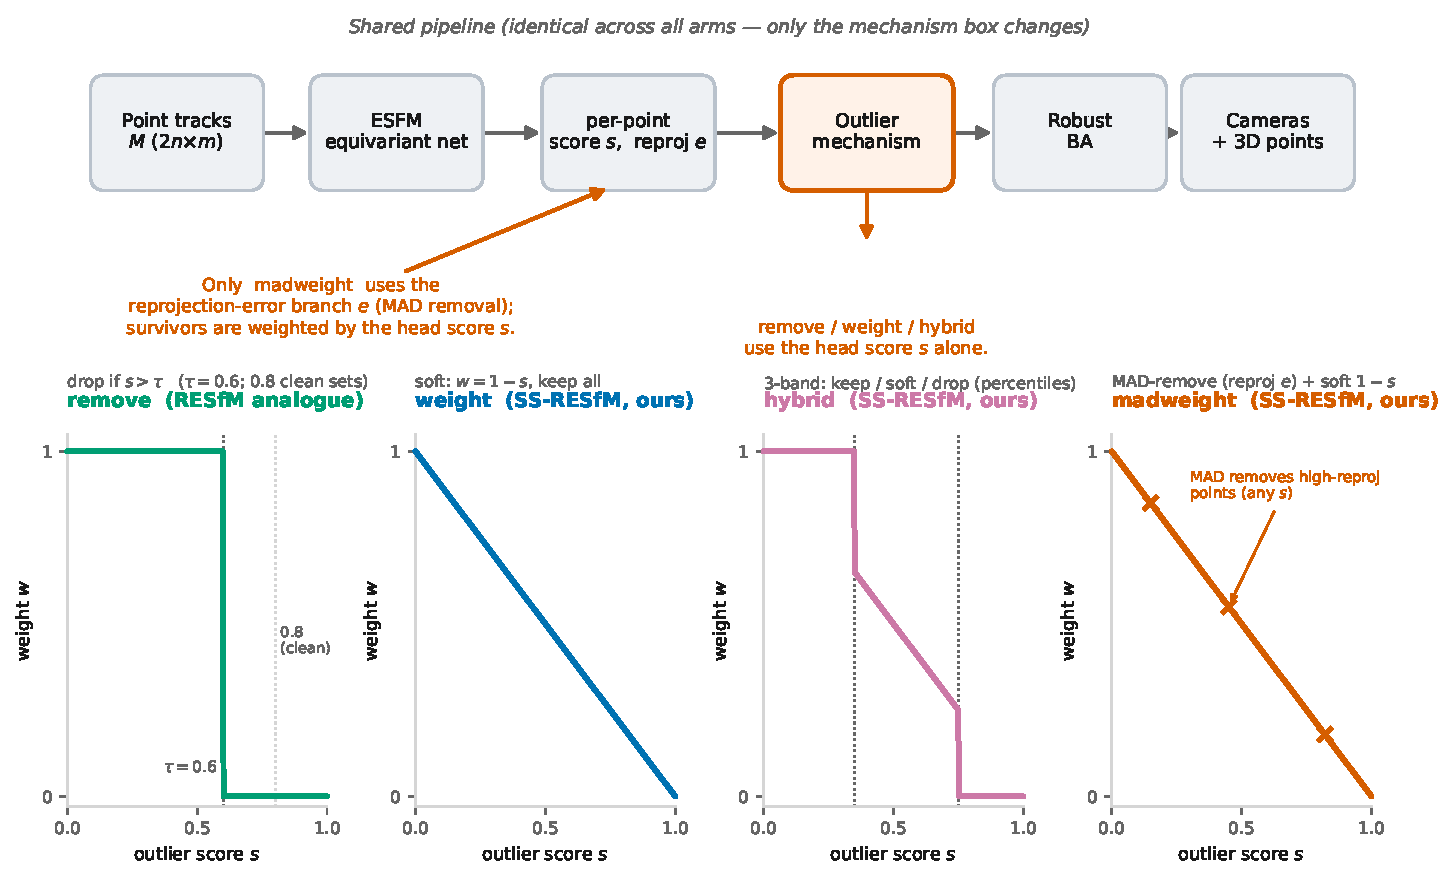
\includegraphics[width=0.85\textwidth]{PATHA_fig2_method.pdf}
\caption{\textbf{Method.} A shared pipeline (top) in which only the outlier-mechanism block
changes. The four mechanisms as weight-vs-signal transfer functions (bottom). Only \mad{}
consumes the reprojection-error branch $e$, and only for its removal step; its surviving
points are still weighted by the head score $s$ ($w{=}1{-}s$). The other three mechanisms
use $s$ alone.}
\label{fig:method}
\end{figure*}

\section{Results}
\subsection{Main comparison}
Table~\ref{tab:main} is the controlled head-to-head under the RESfM-aligned schedule:
every row shares tracks, architecture, schedule, robust BA, and seed, so any difference is
attributable to the outlier mechanism and its supervision alone. Reading along the
contamination axis:
(1)~\emph{Clean OOD} (Olsson $0.5\%$, Strecha $1.7\%$, BlendedMVS $3.1\%$): the
label-free arms win decisively where the supervised head misfires, and the wins are
seed-robust on both sides: every arm beats the full baseline band on BlendedMVS
($0.10$--$0.15$ vs.\ $0.35\pm0.04$; the baseline's rotation failure is $27$--$36\deg$
on every seed) and by ${\sim}3\times$ on Olsson means against four of five baseline
seeds ($3.0\pm0.3$ vs.\ $8.2$--$8.9$; one baseline seed escapes the collapse at $2.69$,
revealing the clean-benchmark failure as basin-dependent rather than universal, its
frequency $4/5$). Strecha is the exception: RESfM's mean is better on every seed
($0.006$--$1.67$ vs.\ $\sim\!2$, though one baseline seed nearly loses it) and the
medians tie ($0.005$).
(2)~\emph{In distribution} (MegaDepth), supervised RESfM retains mean and median.
Its mean is strongly seed-dependent ($0.37\pm0.12$ over five seeds; its best, $0.19$,
approaches the released checkpoint) while its median is stable ($0.07\pm0.02$); the
deterministic self-supervised arms band at $0.50\pm0.08$ and the TTT arm averages
$0.39\pm0.07$ over evaluation repeats; a $\sim\!35\%$ band-level gap without labels,
not a win (though against the authors-faithful configuration, $0.50$, the arms reach
parity).
(3)~\emph{Moderate contamination} (1DSfM, $43\%$) has no stable winner between \mad{}
($11.5\pm2.3$) and the baseline ($10.5\pm1.5$; overlapping bands), so we decline a
directional claim for \mad{}. The \emph{removal family} leads on both statistics in
band terms: remove+TTT $8.9\pm1.2$ vs.\ the baseline's $10.5\pm1.5$ (separated means,
overlapping tails), and plain remove's medians beat \emph{every} baseline seed
pairwise at five seeds each ($1.4$--$1.9$ vs.\ $2.4$--$4.3$; its means, $9.1\pm2.2$,
remain failure-scene-dominated): a label-free win at $43\%$ (Table~\ref{tab:matrix}),
established against the baseline's own five-seed band.
(4)~\emph{Extreme contamination} (1DSfM-hard, ${\sim}60\%$): removal beats weighting
robustly, \mad{} ($18.9\pm4.1$) statistically matches the supervised baseline
($19.2\pm3.4$), and plain remove goes further: $12.4\pm2.1$ over five seeds, below the
baseline on \emph{every} of the $25$ seed pairs (its worst seed, $15.8$, beats the
baseline's best, $16.2$), with tight medians ($10.8\pm2.8$ vs.\ $16.5\pm4.8$); all
label-free arms are far ahead of COLMAP (\S\ref{sec:extreme}). Rotation means (Fig.~\ref{fig:complement}, right) follow the same ordering on
MegaDepth/Strecha/BlendedMVS/Olsson (e.g.\ BlendedMVS $6.6$--$9.6\deg$ self-supervised
vs.\ $36\deg$ supervised) and mildly favor madweight and weight on 1DSfM
($8.3$--$8.4\deg$ vs.\ $9.8\deg$; weight+TTT trails at $11.2\deg$) even where translation
favors the baseline. 

\begin{table*}[t]\centering\small
\caption{\textbf{Main controlled comparison (RESfM-aligned schedule).} Mean\,/\,median
translation error (post-BA), seed 20. All rows share tracks, architecture, schedule,
robust BA, and seed; only the outlier mechanism and its supervision differ. Reference rows
(means) below the rule; upper block = SS-RESfM arms. Best per column in \textbf{bold}. $^{\dagger}$mean$\pm$std over
three evaluation repeats (TTT is run-to-run nondeterministic; appendix).
$^{\ddagger}$mean$\pm$std over seeds $20$--$24$ (both methods). Other cells:
deterministic, seed 20. Lower panels: rotation and registered-camera fraction (metric
priority: translation, then rotation, then $N_r$, following RESfM). ESFM$^{\ast}$:
vanilla ESFM trained and tested on ground-truth-cleaned tracks (clean-track reference;
its mean is failure-scene-dominated, as in RESfM's own Table~1).}
\label{tab:main}
\footnotesize\setlength{\tabcolsep}{3pt}%
\resizebox{\textwidth}{!}{%
\begin{tabular}{lcccccc}
\toprule
Arm & MegaDepth (25.4) & 1DSfM (43.3) & 1DSfM-hard (60) & Strecha (1.7) & BMVS (3.1) & Olsson (0.5)\\
 & $N_c{=}13126$ & $4563$ & $1497$ & $54$ & $225$ & $3858$\\
\midrule
\multicolumn{7}{l}{\emph{Translation error (mean\,/\,median), the primary metric}}\\[1pt]
\mad{}       & 0.422/0.145 & 12.39/4.37 & 18.9$\pm$4.1/$\mathbf{13.4}$$^{\ddagger}$ & 2.50/0.97 & 0.146/$\mathbf{0.004}$ & $\mathbf{3.0\pm 0.3}$/1.4$^{\ddagger}$\\
weight       & 0.423/0.182 & 12.79/11.01 & 22.9$\pm$2.8/15.6$^{\ddagger}$ & 2.00/0.026 & $\mathbf{0.100}$/0.036 & 2.9$\pm$0.3/1.1$^{\ddagger}$\\
weight+TTT   & 0.39$\pm$0.07/0.14$^{\dagger}$ & 16.13/7.16 & 22.2$\pm$3.2/15.3$^{\ddagger}$ & 1.98/$\mathbf{0.005}$ & 0.136/0.011 & 8.0$\pm$0.3/0.6$^{\ddagger}$\\
RESfM-scratch (supervised)$^{\ddagger}$  & $\mathbf{0.37\pm0.12}$/$\mathbf{0.07\pm0.02}$ & $\mathbf{10.5\pm1.5}$/$\mathbf{3.4\pm0.7}$ & 19.2$\pm$3.4/16.5$\pm$4.8 & $\mathbf{0.39\pm0.72/0.01}$ & 0.35$\pm$0.04/0.33 & 7.4$\pm$2.6/0.95\\
\midrule
RESfM (released)            & 0.209 & 10.71 & -- & 0.197 & 0.330 & --\\
RESfM (paper)               & 0.169 & -- & -- & -- & -- & --\\
RESfM-faithful (authors' ckpt selection) & 0.496 & 12.00 & 17.58 & 0.144 & 0.489 & 8.77\\
ESFM$^{\ast}$ (clean tracks) & 0.462 & 13.84 & 15.20 & 1.16 & 0.327 & --\\
\midrule
\multicolumn{7}{l}{\emph{Rotation error ($\deg$, mean\,/\,median), seed 20}}\\[1pt]
\mad{}       & 3.49/1.33 & $\mathbf{8.31}$/4.53 & $\mathbf{14.40}$/$\mathbf{7.39}$ & 14.62/8.43 & 9.60/0.38 & 13.57/4.37\\
weight       & 3.04/1.77 & 8.39/$\mathbf{2.79}$ & 25.58/17.70 & 7.48/0.17 & $\mathbf{6.65}$/3.06 & 13.23/5.41\\
weight+TTT   & 2.51/1.39 & 11.19/11.25 & 31.97/12.83 & 7.41/0.02 & 7.91/$\mathbf{0.55}$ & $\mathbf{10.49}$/$\mathbf{2.27}$\\
RESfM-scratch (supervised)  & $\mathbf{2.01/0.84}$ & 9.79/$\mathbf{2.79}$ & 22.70/15.86 & $\mathbf{0.02/0.01}$ & 36.10/29.55 & 12.34/3.35\\
\midrule
\multicolumn{7}{l}{\emph{Registered cameras $N_r/N_c$, seed 20}}\\[1pt]
\mad{}       & 80\% & 74\% & 38\% & 91\% & $\mathbf{95}$\% & 83\%\\
weight       & 79\% & 77\% & 39\% & 96\% & 88\% & $\mathbf{90}$\%\\
weight+TTT   & 78\% & $\mathbf{80}$\% & $\mathbf{43}$\% & 98\% & $\mathbf{95}$\% & $\mathbf{90}$\%\\
RESfM-scratch (supervised)  & $\mathbf{85}$\% & 77\% & 37\% & $\mathbf{100}$\% & 90\% & 88\%\\
\bottomrule
\end{tabular}}
\end{table*}


\subsection{The complementarity finding}
Fig.~\ref{fig:complement} shows Table~\ref{tab:main} as a picture, and one pattern
organizes it. \emph{Between} supervision regimes, the self-supervised wins concentrate
exactly where a label-free design should help: on clean OOD data, where a classifier
trained on contaminated MegaDepth misfires (on BlendedMVS, RESfM's rotation error explodes
to $36\deg$), and at extreme contamination, where supervision itself can no longer be
manufactured (\S\ref{sec:whyremoval}). \emph{Within} the self-supervised family, the
removal-vs-weighting ordering is monotone in contamination: weighting is best at
$2$--$3\%$, the two tie in distribution, and removal dominates from $43\%$ upward
(\mad{} $12.4$ vs.\ weight $12.8$, plain remove $8.9$, Table~\ref{tab:matrix};
$13.0\pm2.6$ vs.\ $\sim\!22$ at $60\%$). This mechanism-level flip, the answer to our central
question, is stable across schedules and seeds.

\subsection{Learning-rate robustness of the baseline}\label{sec:lrgrid}
Our protocol gives each method its best learning rate at the canonical $20$k budget
($10^{-3}$ for the supervised arms, RESfM's released value; $10^{-4}$ for the
self-supervised arms). To test how much the conclusions depend on this choice we trained
the supervised baseline at $10^{-4}$ as well. In distribution the released value is
clearly right ($0.344$ vs.\ $0.533$), and at $10^{-4}$ the supervised model is
truncation-limited (best checkpoint at the final epoch). Out of distribution, however,
the picture splits: the baseline's Olsson collapse persists at \emph{both} rates
($8.47$ vs.\ $8.54$), i.e.\ the clean-benchmark supervised failure is lr-robust,
whereas its BlendedMVS, 1DSfM, and 1DSfM-hard deficits shrink substantially at the lower
rate ($0.379\!\to\!0.139$, $11.0\!\to\!5.9$, $16.2\!\to\!12.8$): the
under-trained low-rate model overfits MegaDepth less and generalizes better. Two follow-ups
complete the grid. A $30$k-budget replicate at $10^{-4}$ plateaus (best validation at
epoch $16$k, never improving through $30$k), and its evaluation sharpens the picture:
that checkpoint reaches \emph{near-parity in distribution} ($0.365$ vs.\ the $10^{-3}$
baseline's $0.344$) while keeping the OOD gains (1DSfM $6.1$, 1DSfM-hard $13.9$,
BlendedMVS $0.18$), making it the strongest supervised variant out of distribution
(single seed). The Olsson ($8.27$) and Strecha ($1.64$) failures persist, and label-free
plain removal still leads at extreme contamination ($12.4\pm2.1$ vs.\ $13.9$); the OOD
advantage of the low rate is a regularization effect, not an under-training artifact. And the self-supervised
arms show \emph{no} symmetric effect: trained at $10^{-3}$ they are worse on every
dataset (madweight MegaDepth $0.75$ vs.\ $0.42$, 1DSfM $15.7$ vs.\ $12.4$, Olsson
$10.1$ vs.\ $2.6$). Each method's declared rate is therefore its empirical best-of-two,
and the off-rate OOD gain is specific to supervision, consistent with a
COLMAP-label-fitted classifier overfitting in distribution. We scope our claims
accordingly: the Olsson and Strecha findings and the mechanism flip itself are
lr-robust, while the magnitude of the supervised OOD deficit at BlendedMVS and high
contamination depends on the baseline's learning rate.

\subsection{Why label-free removal wins under high contamination}\label{sec:whyremoval}
Two factors explain why the supervised advantage erodes as contamination rises.
First, \emph{domain shift}: the classifier is trained only on in-distribution MegaDepth,
and its decision boundary does not transfer to the outlier statistics of
out-of-distribution internet collections (a domain-shift effect, not a labeling failure:
MegaDepth's labels derive from its curated reference reconstructions, the
trusted-reconstruction condition under which, per Table~\ref{tab:ceiling}, supervision
is sound, and the strong in-distribution result is consistent with this). Second, and more
fundamentally, supervision itself degrades in this regime: RESfM's labeling (Appendix~C
of~\cite{resfm}) assumes a COLMAP reconstruction and ground-truth poses per training
scene: readily obtained for curated data, but exactly what one lacks on the contaminated
collections where robustness is most needed. \mad{} requires neither: it recomputes the
outlier test per-scene from reprojection statistics, so it is unaffected by domain shift
and applicable wherever a partial reconstruction exists. This is why the removal family
prevails at extreme contamination (\S\ref{sec:extreme}); \mad{} shares that robustness
while requiring no learned threshold at all.

\paragraph{Measuring the label ceiling.} We make the second argument quantitative. On $18$
scenes spanning the full contamination axis we simulate the realistic labeling scenario for
a \emph{new} dataset (no ground-truth poses, so labels must come from a from-scratch COLMAP
reconstruction of the same tracks with fixed known intrinsics) and score the resulting
per-observation labels against the ground-truth-pose reference labels
(precision/recall with outlier as the positive class; \emph{coverage} is the fraction of
observations that receive any COLMAP verdict at all, i.e.\ camera registered and track
triangulated; scenes capped at $120$ cameras); Table~\ref{tab:ceiling} reports the
result.
\begin{table}[t]\centering\footnotesize
\caption{\textbf{The label ceiling}: quality of COLMAP-regenerated supervision vs.\
contamination.}
\label{tab:ceiling}
\setlength{\tabcolsep}{3.5pt}%
\begin{tabular}{lccccc}
\toprule
Contam. & $n$ & Cover\% & Prec. & Recall & COLMAP $t$-err\\
\midrule
0--5\%    & 6 & 99.4 & 0.76 & 0.82 & 0.004\\
5--15\%   & 4 & 89.6 & 0.90 & 0.83 & 0.014\\
15--30\%  & 2 & 71.7 & 0.83 & $\mathbf{0.26}$ & 1.02\\
30--45\%  & 3 & 55.7 & 0.74 & $\mathbf{0.39}$ & 0.82\\
45--60\%  & 3 & 55.1 & 0.87 & $\mathbf{0.39}$ & 11.0\\
\bottomrule
\end{tabular}
\end{table}
Precision stays high throughout, but \emph{recall collapses} from $0.82$ to
$0.26$--$0.39$ and coverage halves once contamination exceeds ${\sim}15\%$: the corrupted
reconstruction absorbs enough outliers that most reproject acceptably under its distorted
geometry, and half the observations receive no label at all. A head trained on such labels
is actively taught that most true outliers are inliers, precisely where robustness
matters. Conversely, below ${\sim}15\%$ COLMAP-derived labels are excellent, consistent
with RESfM's strong in-distribution result and delimiting where the supervised recipe is
sound.

\subsection{Extreme contamination: the 1DSfM-hard set}\label{sec:extreme}
To probe beyond 1DSfM's $43\%$, we evaluate on the five held-out 1DSfM-hard scenes
($\sim\!60\%$ measured contamination, $300$ cameras each). The learned arms are those of
Table~\ref{tab:main} (this restates its 1DSfM-hard column alongside rotation), and
COLMAP runs incremental mapping on the same tracks with known intrinsics
(Table~\ref{tab:hard}).
\begin{table}[t]\centering\small
\caption{\textbf{1DSfM-hard} ($\sim\!60\%$ outliers, seed 20): translation/rotation
and registered fraction.}
\label{tab:hard}
\begin{tabular}{lcc}
\toprule
Method & Trans/Rot (post-BA) & Registered\\
\midrule
remove & $\mathbf{10.6}$/$\mathbf{12.4}$ & all\\
\mad{} & 12.2/14.4 & all\\
remove+TTT & 15.2/16.8 & all\\
RESfM-scratch              & 16.2/22.7 & all\\
huberweight & 16.9/24.5 & all\\
COLMAP                     & 20.9/--   & 64\%\\
weight & 21.9/25.6 & all\\
stdweight & 23.2/27.3 & all\\
hybrid & 26.3/28.7 & all\\
weight+TTT & 26.4/32.0 & all\\
\bottomrule
\end{tabular}
\end{table}
The mechanism-level ordering extrapolates: over seeds $20$--$22$, plain remove attains
$13.0\pm2.6$ translation (below the supervised $16.2$, seed 20, on every seed; medians
$11.9\pm0.6$ vs.\ $13.1$), \mad{} at $17.0\pm4.4$ statistically matches it, every other mechanism (soft, hybrid, and alternative robust
statistics) lands at $16.9$ or worse (Table~\ref{tab:hard}), and COLMAP degrades severely: its error is computed
\emph{only over the $64\%$ of cameras it registers} (a favorable metric) yet still loses.
Errors are large for every method (these scenes are hard), but the trend matches the
label-ceiling prediction: the supervised advantage vanishes exactly where supervision can
no longer be manufactured.



\subsection{Full mechanism matrix}
Table~\ref{tab:matrix} completes the mechanism study (all arms, RESfM-aligned schedule,
seed 20). Notably, at $43\%$ the \emph{plain-removal} family leads every arm including the
supervised baseline, and the full three-seed band confirms it: remove+TTT
$8.7\pm1.1$ mean (every seed below the baseline's $11.0$), plain remove median
$1.59\pm0.18$ (vs.\ $2.9$; means $9.1\pm2.8$, dominated by the two failure scenes). On
clean data the soft arms dominate the removal family, reproducing the complementarity.
On outlier-free Olsson the grid flattens (all label-free arms $2.6$--$4.1$ vs.\
supervised $8.5$): the clean-benchmark failure is specific to the supervised head, not
the mechanism.

\begin{table}[t]\centering\scriptsize
\setlength{\tabcolsep}{2.5pt}%
\caption{\textbf{Full shallow mechanism matrix} (RESfM-aligned schedule, seed 20;
$^{\ddagger}$mean$\pm$std over seeds 20--22). Mean\,/\,median translation
(post-BA); Olsson column: means. Best per column in \textbf{bold}.}
\label{tab:matrix}
\resizebox{\linewidth}{!}{%
\begin{tabular}{lccccc}
\toprule
Arm & MD & 1DSfM & Strecha & BMVS & Olsson\\
\midrule
remove       & 0.60/0.19 & 9.1$\pm$2.8/$\mathbf{1.6\pm 0.2}$$^{\ddagger}$ & 3.02/1.68 & 0.27/0.19 & 2.81\\
remove+TTT   & 0.49/0.13 & $\mathbf{8.7\pm 1.1}$/2.2$\pm$1.1$^{\ddagger}$ & 2.97/1.56 & 0.19/0.07 & 4.07\\
hybrid       & 0.37/0.20 & 16.0$\pm$1.4/6.7$\pm$4.4$^{\ddagger}$ & 2.70/1.39 & 0.10/0.03 & 2.82\\
hybrid+TTT   & 0.39/0.14 & 15.4$\pm$1.1/10.7$\pm$3.5$^{\ddagger}$ & 3.52/2.65 & 0.13/$\mathbf{0.00}$ & 3.19\\
\mad{}       & 0.42/0.15 & 11.5$\pm$2.3/6.0$\pm$1.4$^{\ddagger}$ & 2.50/0.97 & 0.15/0.004 & $\mathbf{2.57}$\\
weight       & 0.42/0.18 & 15.8$\pm$3.1/10.9$\pm$2.1$^{\ddagger}$ & 2.00/0.03 & $\mathbf{0.10}$/0.04 & 2.65\\
weight+TTT   & 0.39/0.14 & 17.0$\pm$1.3/10.9$\pm$4.1$^{\ddagger}$ & 1.98/$\mathbf{0.005}$ & 0.14/0.01 & 7.74\\
\midrule
RESfM (sup.) & $\mathbf{0.34/0.07}$ & 11.03/2.93 & $\mathbf{0.006/0.005}$ & 0.38/0.35 & 8.47\\
\bottomrule
\end{tabular}}%
\end{table}

\subsection{Which robust statistic? MAD vs.\ STD vs.\ Huber}
\mad{} removes by a robust statistic of the reprojection error; we ablate the statistic
holding the head reweighting fixed: MAD (median${}+\alpha\cdot1.4826\,$MAD, $50\%$
breakdown), a Huber M-estimate of scale (IRLS), and non-robust STD
(mean${}+\alpha\sigma$), all at $\alpha{=}2$. Table~\ref{tab:madstat} reports the
ablation over seeds $20$--$22$: only MAD's 1DSfM median is stable; Huber's collapses on
one seed, and non-robust STD is consistently poor, its mean/$\sigma$ threshold inflated
by the very outliers it should catch. On clean data all three are comparable: little is
removed either way, the right behavior without outliers. The $50\%$-breakdown statistic
is the only reliably robust choice, and we use MAD in \mad{}.

\begin{table}[t]\centering\scriptsize
\setlength{\tabcolsep}{2.5pt}%
\caption{\textbf{Removal-statistic ablation} (head reweighting fixed). Only MAD's
median is seed-stable.}
\label{tab:madstat}
\begin{tabular}{lccc}
\toprule
Statistic & 1DSfM mean & 1DSfM med.\ s20/21/22 & BMVS\\
\midrule
MAD (\mad{}) & 11.5$\pm$2.3 & $\mathbf{4.4\,/\,7.0\,/\,6.6}$ & 0.15\\
Huber & $\mathbf{11.5\pm 1.6}$ & 3.8 / 12.4 / 5.3 & $\mathbf{0.11}$\\
STD & 15.2$\pm$1.2 & 13.3 / 9.0 / 12.9 & 0.15\\
\bottomrule
\end{tabular}
\end{table}

\subsection{Per-scene complementarity and the limits of contamination-based selection}
Fig.~\ref{fig:perscene} tests the flip \emph{per scene}: each scene's outlier rate vs.\
the signed advantage of the best removal mechanism over soft weighting. On OOD data,
weight wins the low-contamination scenes and removal the high-contamination ones; the
crossover is bracketed to the sparsely-sampled ${\sim}3$--$29\%$ band.

\begin{figure}[t]
\centering
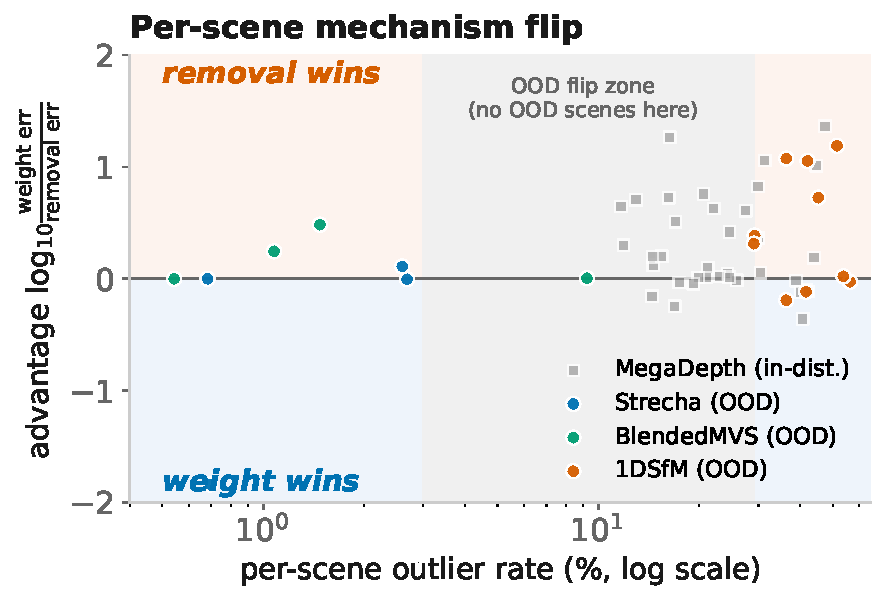
\includegraphics[width=\linewidth]{PATHA_fig4_perscene.pdf}
\caption{\textbf{Per-scene complementarity} (RESfM-aligned schedule). Each point is one
scene: outlier rate (x, log) vs.\ signed advantage of removal over soft weighting. Weight
wins at low contamination, removal at high contamination.}
\label{fig:perscene}
\end{figure}

\noindent\textbf{Does per-scene contamination help selection?} No: within each dataset
contamination is too homogeneous to trigger different choices, so a contamination-keyed
selector (\mad{} if scene rate ${\ge}10\%$, else weight) collapses to per-dataset
selection (Table~\ref{tab:selector}). An \emph{oracle} choosing the best of five
mechanisms per scene from ground-truth error would change the picture: MegaDepth
$0.42\!\to\!0.116$, surpassing every fixed arm, the supervised baseline at $0.344$,
and even RESfM-released at $0.209$, and 1DSfM $12.4\!\to\!5.8$ vs.\ the
baseline's $11.0$. The performance is thus already \emph{latent} in the label-free mechanism family;
selection, not mechanism design, is the bottleneck, and realizing this headroom without
ground truth is future work.

\begin{table}[t]\centering\footnotesize
\setlength{\tabcolsep}{3pt}%
\caption{\textbf{Per-scene selection} (mean translation; RESfM-aligned schedule).
Contamination-keyed selection collapses to per-dataset choice. The oracle uses
ground-truth error over five mechanisms: an upper bound, not a deployable method.}
\label{tab:selector}
\begin{tabular}{lcccc}
\toprule
Dataset & weight & madwt & contam & oracle (GT)\\
\midrule
MegaDepth  & 0.423 & $\mathbf{0.422}$ & 0.422 & $\mathit{0.116}$\\
1DSfM      & 12.79 & $\mathbf{12.39}$ & 12.39 & $\mathit{5.78}$\\
Strecha    & $\mathbf{2.00}$ & 2.50 & 2.00 & $\mathit{1.98}$\\
BlendedMVS & $\mathbf{0.100}$ & 0.146 & 0.100 & $\mathit{0.083}$\\
\bottomrule
\end{tabular}
\end{table}

\subsection{Qualitative}
Fig.~\ref{fig:qual} overlays BA-aligned camera centers on ground truth for 1DSfM
NYC\_Library. Label-free \mad{} ($2.94$) leaves far fewer gross-drift cameras than the
supervised from-scratch baseline ($6.28$), which shows more and larger gross drifts.

\begin{figure}[t]
\centering
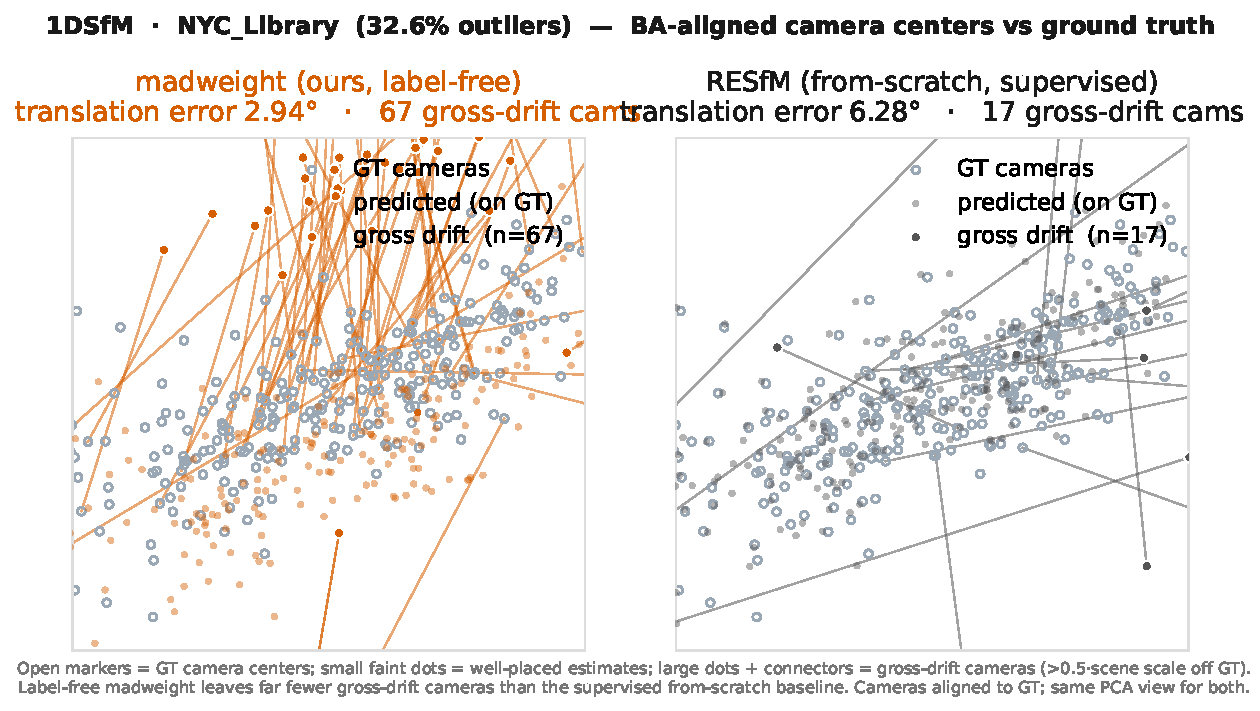
\includegraphics[width=\linewidth]{PATHA_fig3_qualitative.pdf}
\caption{\textbf{Qualitative 1DSfM (NYC\_Library, 32.6\% outliers).} BA-aligned camera
centers vs.\ GT (open markers); large dots\,+\,connectors mark gross-drift cameras. \mad{}
(left, $2.94$) has fewer and shorter drifts than RESfM-from-scratch (right, $6.28$).}
\label{fig:qual}
\end{figure}

\subsection{Preliminary: training-pool diversity and the label ceiling}
A preliminary experiment (single seed, under a coarser five-milestone decay schedule;
cf.\ \S\ref{sec:protocol}) retrains both methods on progressively diversified pools: MegaDepth-27
$\to$ $+$ETH3D ($39$ scenes, added data ${\sim}8\%$ contaminated) $\to$ $+$VGG/T\&T ($52$
scenes, adding a ${\sim}16\%$-contaminated mid-band). The supervised baseline's clean-OOD
accuracy degrades \emph{monotonically} with diversity (Strecha
$0.006\!\to\!0.77\!\to\!2.83$); in distribution the same diversification is nearly
free (MegaDepth $0.33\!\to\!0.32\!\to\!0.44$, the first step within noise), so the
collapse is specific to clean OOD generalization, not a general capacity cost. Meanwhile the clean addition yielded no high-contamination
gain and only the contaminated mid-band coincided with one (1DSfM $11.0/11.5/8.8$;
differences within single-seed noise on this benchmark, so consistent with, though not
established by, these runs). If it holds, the implication is pointed: the data that
helps is precisely the data whose COLMAP labels degrade (cf.\ the label ceiling), making
supervised diversity scaling self-limiting. The
label-free arms diverge by mechanism: soft weighting collapses on clean OOD like the
baseline (BlendedMVS $2.9$--$4.0$), whereas \mad{} is diversity-robust (BlendedMVS
$0.22$--$0.30$) and reaches our best high-contamination result anywhere (1DSfM $6.4$ at
$52$ scenes). We report this as a labeled preliminary observation; a canonical-schedule,
multi-seed replication is in progress.

\section{Limitations}
(1)~No single deployable configuration wins all datasets; selecting the best mechanism per
dataset (Table~\ref{tab:main}) requires knowing the contamination level. We present a study
of the phenomenon, not a turnkey adaptive method; an unsupervised selector is future work.
(2)~Supervised RESfM retains in-distribution MegaDepth (the self-supervised arms come
within $\sim\!13$--$23\%$, no closer) and the clean Strecha mean, and RESfM-released
remains stronger on MegaDepth, so we claim no SOTA. (3)~Versus supervision, \mad{} has no stable winner at moderate ($11.5\pm2.3$ vs.\
$10.1\pm0.9$) or extreme ($17.0\pm4.4$ vs.\ $17.3\pm1.6$) contamination; plain
remove leads every baseline seed pairwise at $\sim\!60\%$ and on medians at $43\%$,
its means at $43\%$ separating from the baseline band without full pairwise dominance;
and plain removal's wins come over a reduced registered-camera set
(\S\ref{sec:protocol}). (3b)~The magnitude of the supervised OOD deficit at BlendedMVS
and high contamination is learning-rate-dependent (\S\ref{sec:lrgrid}); the Olsson
collapse and the mechanism flip are not.
(4)~OOD tracks are self-constructed; OOD numbers are controlled within our pipeline
and not comparable to RESfM's published OOD numbers. (5)~Two symmetric-structure scenes (Ellis Island, Tower of London) fail for all
methods and inflate 1DSfM means; these are the cases where excess removal can disconnect
the viewing graph~\cite{resfm}.

\section{Conclusion}
SS-RESfM shows that deep SfM outlier handling can be made \emph{entirely
self-supervised} while staying within
$\sim\!13$--$23\%$ of the supervised baseline in distribution, winning two of the three
clean-OOD splits, and beating it at high contamination (plain removal below the baseline on every
seed), where both beat COLMAP and supervision itself can no longer be manufactured. The optimal mechanism is contamination-dependent:
removal at high contamination, reweighting at low. Robust deep SfM should treat outlier
handling as adaptive and self-supervised; code, configurations, and the rebuilt OOD
tracks will be released upon publication.

\label{sec:endcontent}%
\begin{thebibliography}{99}\small

\bibitem[Khatib et al.(2025)]{resfm} Khatib, Kasten, Moran, Galun, and Basri. RESfM: Robust Deep Equivariant Structure from Motion. ICLR 2025.

\bibitem[Moran et al.(2021)]{esfm} Moran, Koslowsky, Kasten, Maron, Galun, and Basri. Deep Permutation Equivariant Structure from Motion. ICCV 2021.

\bibitem[Brynte et al.(2024)]{gasfm} Brynte, Iglesias, Olsson, and Kahl. Learning Structure-from-Motion with Graph Attention Networks. CVPR 2024.

\bibitem[Sch\"onberger and Frahm(2016)]{colmap} Sch\"onberger and Frahm. Structure-from-Motion Revisited. CVPR 2016.

\bibitem[Rousseeuw and Croux(1993)]{mad} Rousseeuw and Croux. Alternatives to the Median Absolute Deviation. JASA 1993.

\bibitem[Wilson and Snavely(2014)]{onedsfm} Wilson and Snavely. Robust Global Translations with 1DSfM. ECCV 2014.

\bibitem[Li and Snavely(2018)]{megadepth} Li and Snavely. MegaDepth: Learning Single-View Depth Prediction from Internet Photos. CVPR 2018.

\bibitem[Strecha et al.(2008)]{strecha} Strecha, von Hansen, Van Gool, Fua, and Thoennessen. On Benchmarking Camera Calibration and Multi-View Stereo for High-Resolution Imagery. CVPR 2008.

\bibitem[Yao et al.(2020)]{blendedmvs} Yao et al. BlendedMVS: A Large-Scale Dataset for Generalized Multi-View Stereo Networks. CVPR 2020.

\bibitem[Olsson and Enqvist(2011)]{olsson} Olsson and Enqvist. Stable Structure from Motion for Unordered Image Collections. SCIA 2011.

\end{thebibliography}

\end{document}
